\section{Simulated serological data from \texttt{serosim}\cite{Menezes2023-ti}}

\begin{figure}[h]
    \centering
    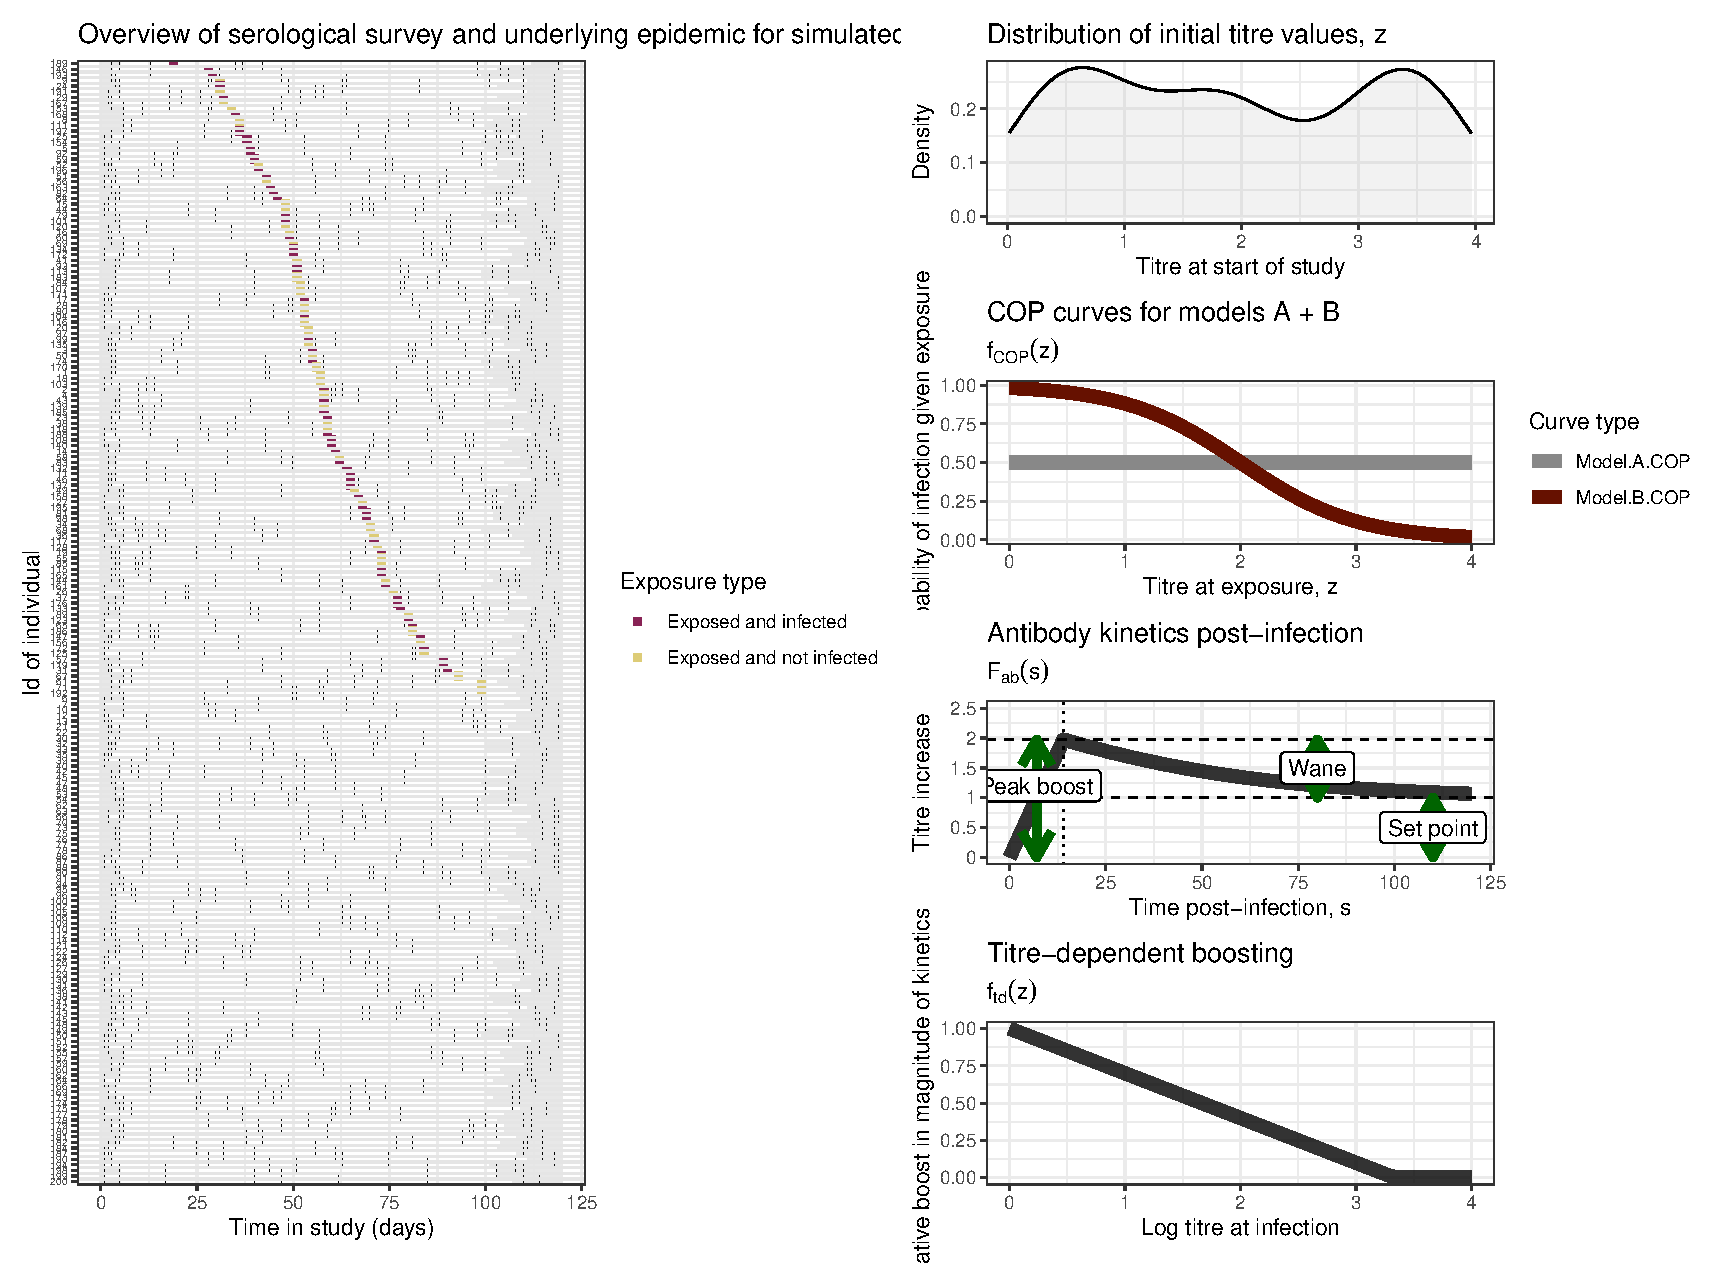
\includegraphics[width=1\textwidth]{\myimagepath/outputs/sim_data/summary_fig_A_CES.pdf}     \caption{Schematics showing the simulated data structure from \texttt{serosim}\cite{Menezes2023-ti}}
    \label{fig:sim_A}
\end{figure}

\paragraph{}We simulate serological data using the \texttt{serosim}\cite{Menezes2023-ti} R package to demonstrate our modelling framework's capabilities at simulation recovery. We simulate continuous epidemic serosurveillence (CES) cohort data, which represents a serostudy in which individuals are followed over an epidemic wave and bled at multiple random time points throughout. The simulated data includes $M = 200$ individuals with serological samples taken within the first seven days of the study's starting and a sample within the last seven days of the study's ending. These individuals also had three samples taken randomly throughout the study (over the 120-day epidemic wave). Each individual has a 60\% chance of exposure to the virus over the study timeframe and can have a maximum of one exposure. To model an even epidemic peak, we simulate the exposure time for each individual from a normal distribution, $\mathcal{N}(60, 20)$ days. A figure showing the timing of the bleeds, infections and exposures and the starting titre values for each individual is given in \textbf{Figure~\ref{fig:sim_A}A-B}.

\paragraph{}We define the correlate of protection (COP) as the probability of infection given a titre value at exposure. Data are simulated with two different correlates of protection; one is uniform at 50\% for all titres at exposure (COP model A) and thus represents no titre-dependent COP. The second follows a logistic distribution (COP model B) of the form:

\begin{equation}
\label{eq_cop}
f_{cop}(x, \beta_0, \beta_1) = \frac{1}{1 + \exp(- (\beta_0 + \beta_1x))}
\end{equation}

where $\beta_0 = -4$ and $\beta_1 = 2$ in the simulated data and $x$ is the titre value at exposure. This represents a pathogen for which higher antibody titres are associated with higher levels of protection from infection. Note in these data, we assume antibody trajectories remain constant until the timing of infection, such $f_{cop}(X_{j, t}, \beta_0, \beta_1) = f_{cop}(Z^0_{j}, \beta_0, \beta_1)$ where $Z^0_{j}$ is the antibody titre of an individual at their first bleed at the start of the study.  A figure showing the two COP models is given in \textbf{Figure~\ref{fig:sim_A}C}.


\paragraph{}Following infection, the antibody kinetics are assumed to follow a linear rise to a peak at 14 days, followed by an exponential decay to a set-point value.\cite{Srivastava2023-of} The formula for this biphasic trajectory is given by \textbf{Equation~\ref{eq_ab}}.

\begin{equation}
\label{eq_ab}
f^1_{ab}(s, a, b, c) =
\begin{cases}
  \ln(\exp(a) + \exp(b)) / 14, & \text{if }s \leq 14 \\
  \ln(\exp(a) \exp(-(b/10)(t - 14)) + \exp(c)), &\text{if } s > 14
\end{cases}
\end{equation}

where $a = 1.5$, $b = 2$, and $c = 1$ are values in the simulated data (\textbf{Figure~\ref{fig:sim_A}D}) and $s$ is the number of days post infection. We also assume that the magnitude of these dynamics depends on pre-existing titre values, with higher pre-existing values seeing attenuated dynamics relative to lower pre-existing tire values. The titre-dependent boosting is assumed to follow a linear decay truncated at 0, that is, given a titre value $z$, $f^2_{ab}(Z_j^0, \alpha) = \max(1 - \alpha z, 0)$. where $\alpha = 0.3$ in the simulated data (\textbf{Figure~\ref{fig:sim_A}E}). Therefore, the model estimated titre value at time $t$ for individual $j$, given time $s$ since infection with a titre value at infection of $Z_{j}^0$, is given by;  

\begin{equation}
\label{eq_ab2}
f_{ab}(s, Z^0_{j}, a, b, c, \alpha) = f^1_{ab}(s, a, b, c)f^2_{ab}(Z^0_{j}, \alpha) 
\end{equation}


\begin{figure}[h]
    \centering
    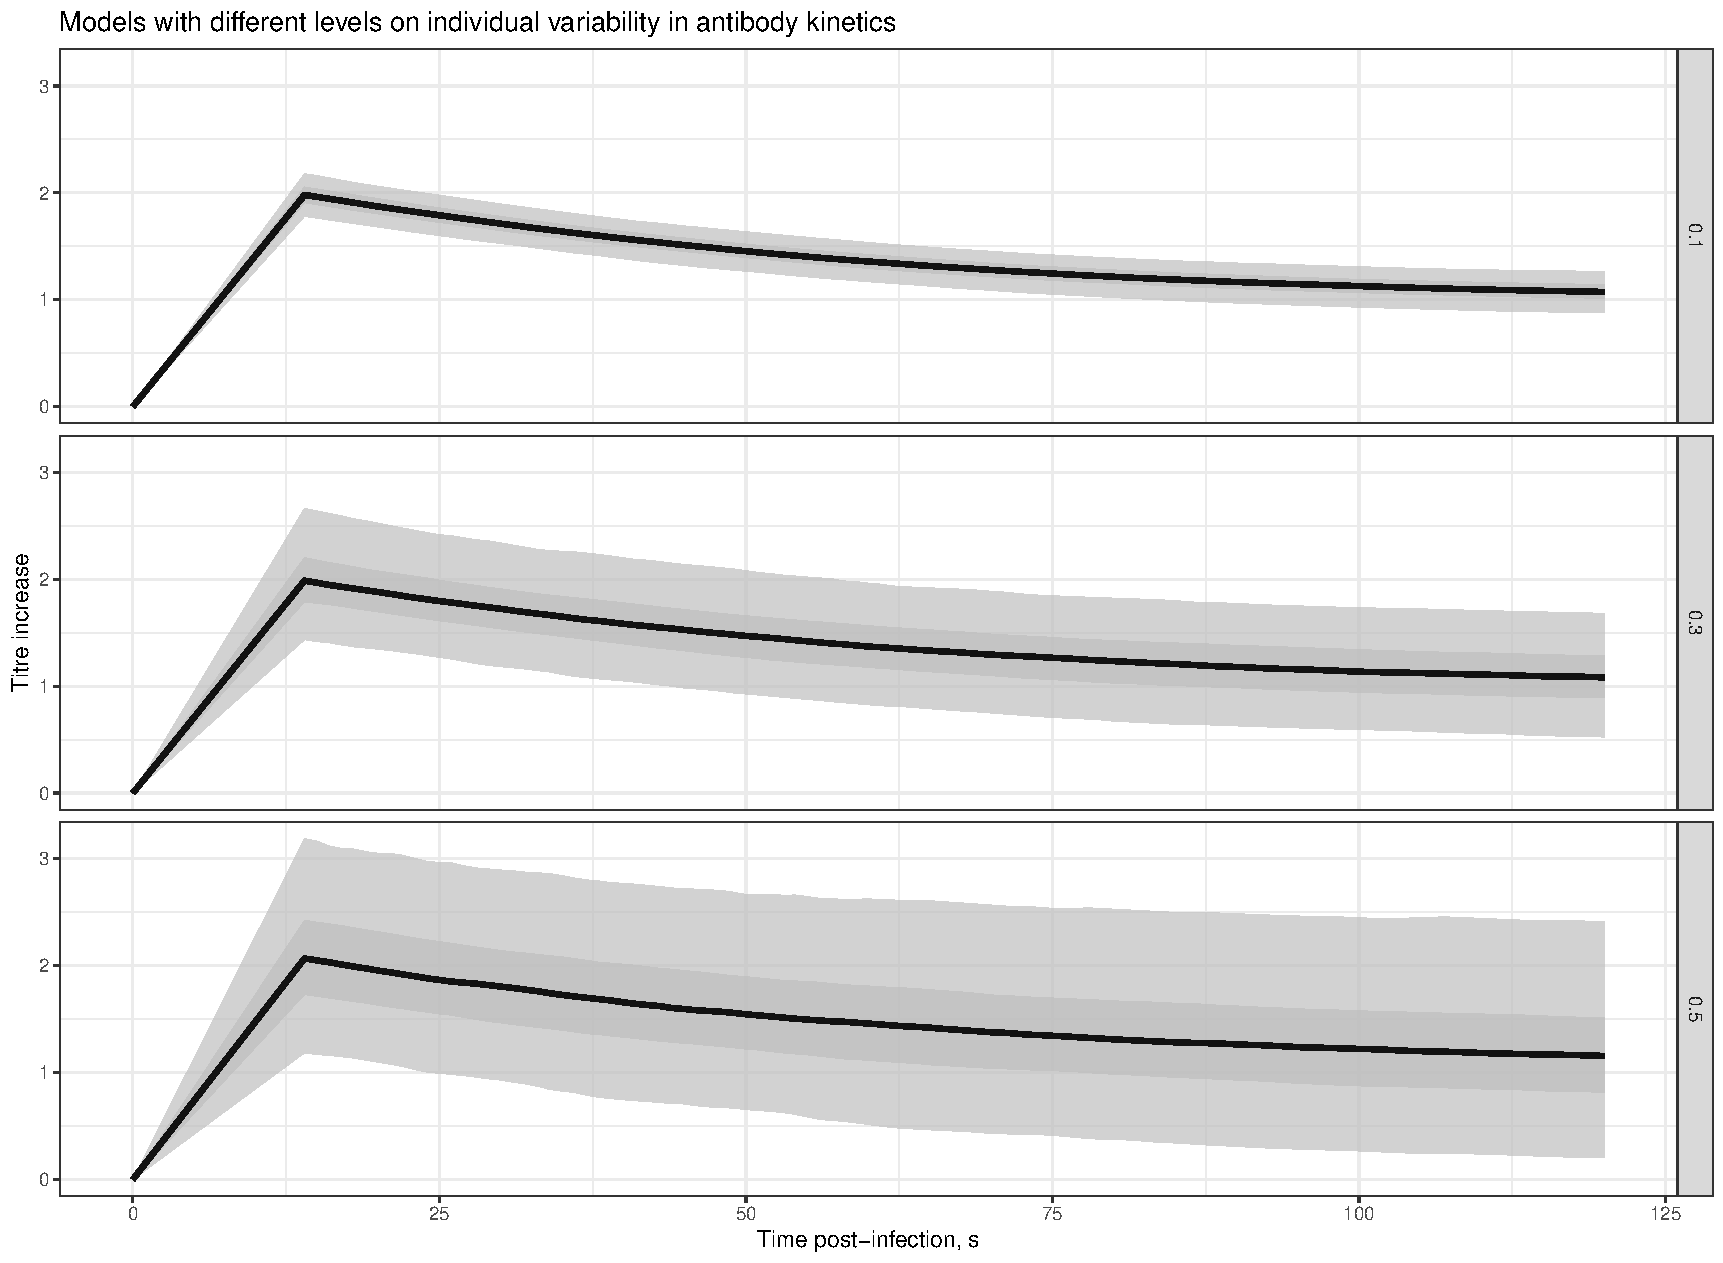
\includegraphics[width=1\textwidth]{\myimagepath/outputs/sim_data/summary_fig_B_CES.pdf}     \caption{Schematics showing three levels of individual-level uncertainty and the impact on the variability of antibody kinetics.}
    \label{fig:sim_B}
\end{figure}

t
\paragraph{}To model heterogeneity in individual-level antibody kinetics, we simulate $a, b, c$, and $\alpha$ from normal distributions where the mean $\mu$ is their simulated values and the standard deviation given by $\mu\sigma^*$. We simulate three levels of uncertainty for $\sigma^* = \{0.1, 0.3, 0.5\}$ for both of the COP models, giving six simulated datasets. A schematic showing how these levels of uncertainty influence the variability of the antibody kinetics trajectories is shown in \textbf{Figure~\ref{fig:sim_B}}. We will fit the to-be-described methods to these datasets and explore how the correlate of protection and level of variability in antibody kinetics impacts the framework's ability to recover simulated data. 

We note that the simulated data for the correlate of protection does not exactly match the functional form chosen when inferred from the infected population. We plot the realised COP simulated curve and compare it to the functional COP curve in \textbf{Figure~\ref{fig:sim_C}}. A summary of the parameter values and functions used to generate the simulated data can be found in \textbf{Table~\ref{table:not_sim}}.

\begin{figure}[h]
    \centering
    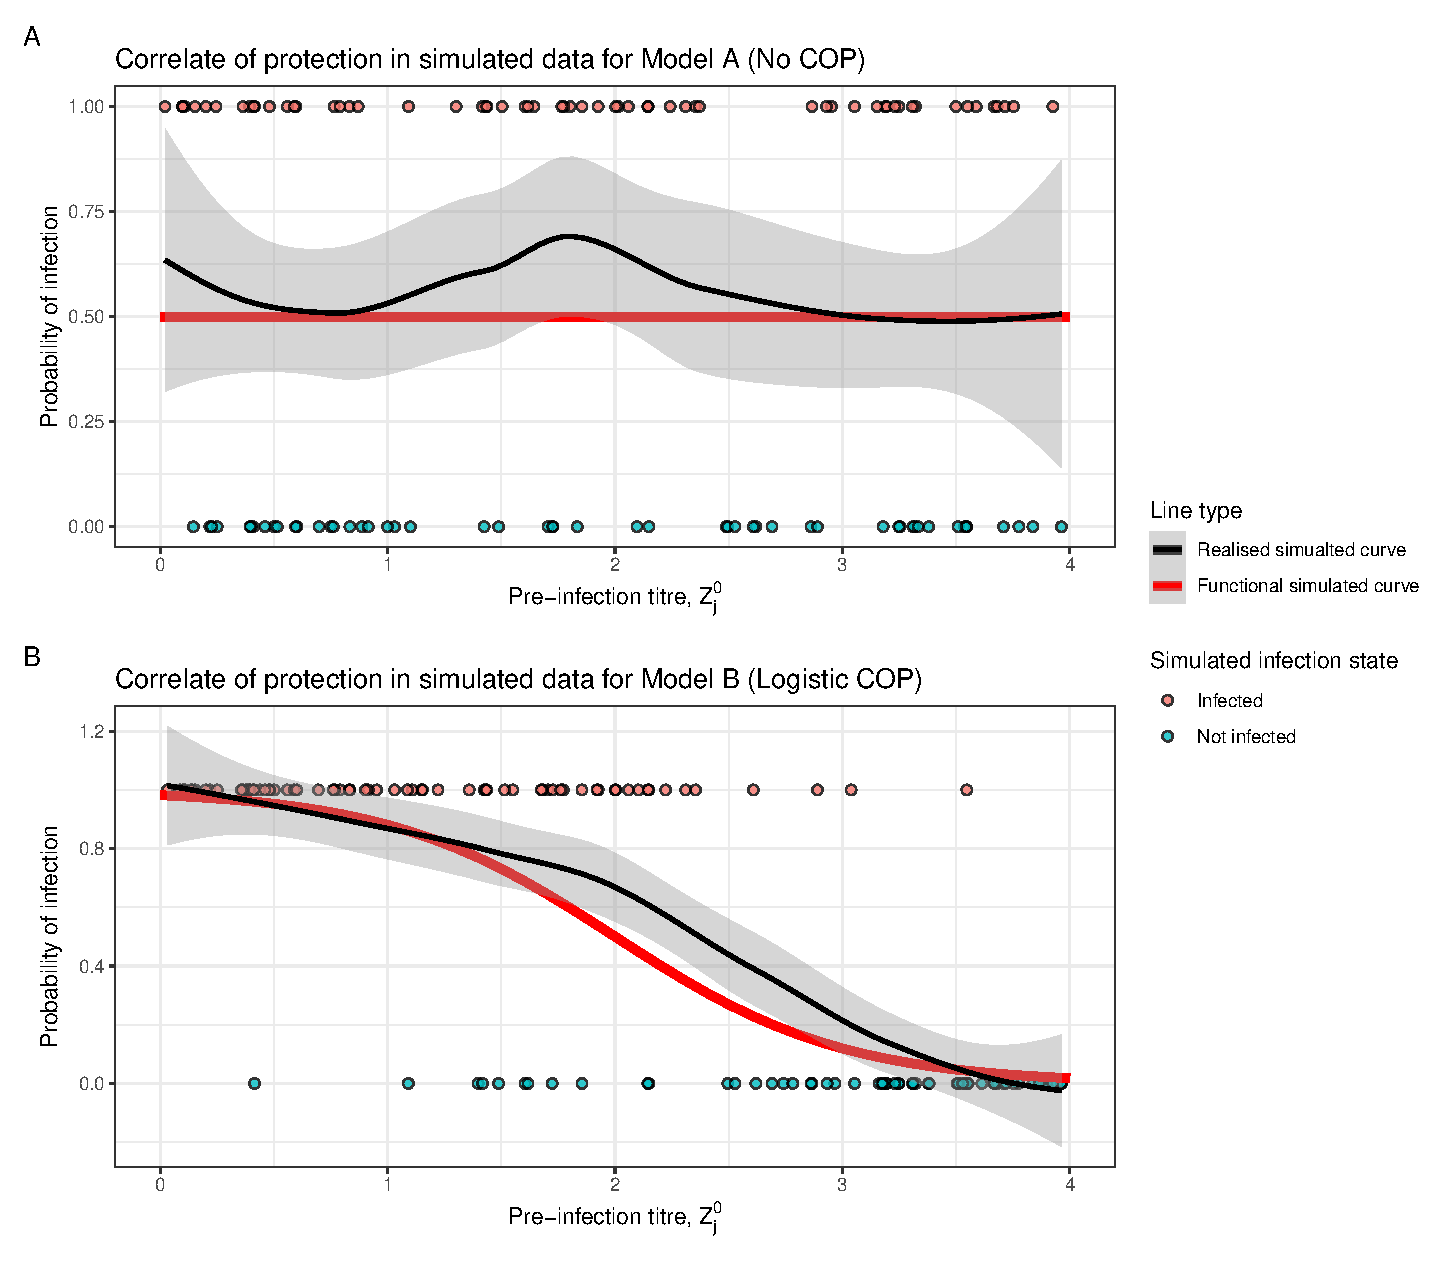
\includegraphics[width=1\textwidth]{\myimagepath/outputs/sim_data/summary_fig_C_CES.pdf}     \caption{Schematics showing the difference between the functional form chosen to simulate the COP and the recovered COP from the exposed individuals.   }
    \label{fig:sim_C}
\end{figure}

\begin{table}[H]
    \centering
    \begin{tabular}{|c|l| l| }
         \hline
        \textbf{Symbol} & \textbf{Description} & \textbf{Value}\\
        \hline
         $M$ & Number of individuals in the sample, we use subscript $j$ to refer to an individual.& 200 \\ \hline
         $T$ & Time over which the study is run.  & 120 days \\ \hline         
         $P(E_j)$ & Probability of exposure for individual $j$ over time period.  & 60\% \\ \hline
         $E^\tau_j$ & Timing of exposure for exposed individuals.  & $\mathcal{N}(60, 20)$ \\ \hline
         $a$ & Parameter describing the peak boost of the post-infection antibody kinetics   & 1.5 \\ \hline
         $b$ &  Parameter describing the waning rate of the post-infection antibody kinetics &  2\\ \hline
         $c$ & Parameter describing the set-point value of the post-infection antibody kinetics & 1 \\ \hline
         $\alpha$ &  Parameter describing the titre-dependent boosting of the antibody kinetics & 0.3 \\ \hline
         $\beta_0$ & Intercept parameter of the logistic function for the COP  & -4 \\ \hline
         $\beta_1$&  Slope parameter of the logistic function for the COP  &  2 \\ \hline
         $f_{ab}$ & Antibody kinetics function & \textbf{Equation~\ref{eq_ab2}} \\ \hline         
         $f_{cop}$ & Logistic correlate of protection  & \textbf{Equation~\ref{eq_cop}} \\ \hline
    \end{tabular}
    \caption{Table of parameters associated with the simulated data and their values}
   	\label{table:not_sim}
\end{table}